% !TEX root = ../Robotik.tex
\chapter{Probabilistische Methoden und Kartierungen}
\section{Problemstellung}

\begin{description}
	\item[Sensordaten] Roboter empfängt regelmäßig Sensordaten, jedoch mit
		Unsicherheit behaftet.
	\item[Steuerdaten] Roboter führt regelmäßig Bewegungen mit Steuerdaten $u_k$
		durch, aber diese entsprechen nicht exakt den vorgegebenen Steuerdaten.
	\item[Position und Umgebungsmodell] Position schätzt seine globale Position
		aufgrund der Sensor- und Steuerdaten in seiner Umgebungskarte, jedoch auch
		mit Unsicherheit behaftet
\end{description}

\section{Modellierung von Unsicherheit}
Die Unsicherheiten werden mit Wahrscheinlichkeiten modelliert. So kann der
Zustand von dynamsichen Systemen probabilistisch geschätzt werden.

\paragraph{Beispiel: Localization beim Roboter}
Dabei wird die Position ermittelt an der sich der Roboter am
wahrscheinlichsten befindet. Die Lokalisierung wird somit zu einem
Wahrscheinlichkeitsdichte Problem bei dem alle vorangegangenen Sensorwerte
berücksichtigt werden.

\section{Umgebungsmodellierung mit Occupancy Grids}
\subsection{Satz von Bayes}
\begin{align*}
	p(A) &= \text{Wahrscheinlichkeit das die Aussage } A \text{ zutrifft} \\
	P(A|B) &= \text{Wahrscheinlichkeit, dass } p(A) \text{ unter der
									Voraussetzung das }B\text{ gilt} \\
  P(A|B) &= p(B|A) * \frac{p(A)}{p(B)}
\end{align*}

\subsection{Evidence Grids (Beweisraster)}
\textbf{Problem}: reale Sensordaten erhalten häufig Rauschen.
Rauschen bei  Sensordaten führt zu Abweichungen des Idealwerts $\Rightarrow$
schwerwiegende Fehler.

Im Gegensatz zu Occupancy Grids nutzen Evidence Grids keine Binärwerte um die
Belegung darzustellen. Sie sammeln Beweismittel und geben die
Wahrscheinlichkeit für die Belegung jeder Zelle an:
$$
	Z(x,y) = p(Z_{x,y,belegt} | Sensorwert) / p(Z_{x,y,frei} | Sensorwert)
$$
Da die Wahrscheinlichkeit für die Belegung unter einem bestimmten Sensorwert
schwer zu berechnen ist wird der Satz von Bayes benutzt:
$$
	Z(x,y) = \frac{p(Sensorwert | Z_{x,y,belegt}) * p(Z_{x,y,belegt})}
								{p(Sensorwert | Z_{x,y,frei}) * P(Z_{x,y,frei})}
$$
Beim Start der Erstellung wird angenommen, dass die Wahrscheinlichkeit für die
Belegung einer Zelle bei 50\% liegt. Dannach wird die Wahrscheinlichkeit
fortlaufend mit den aktuellen Sensorwerten aktualisiert.

Die direkte Anwendung des Bayessischen Filters auf das
Selbstlokalisierungsproblem ergibt sich die sogenannte \textbf{Markov-
Lokalisierung}

\section{Bayes-Filter Algorithmus}
Der Vertrauenszustand (\textbf{belief}) spiegelt internes Wissen des Roboters
über den Zustand seiner Umgebung wieder.

\subsection{Algorithmus}
Ein Rekursiver Algorithmus der aus dem vorangegangenen Status den neuen
berechnet:
\begin{align*}
	z_t &= \text{Observationsmesswert, aktuelle Sensorwerte der Umgebung} \\
	u_t &= \text{Aktionsmesswert, aktuelle Zustandsänderungen im Interval }
		]t-1, t] \\
	x_t &= \text{Zustand zum Zeintpunkt }t \\
	bel(x_t) &= p(x_t | Z_{1:t}, u_{1:t}) \\
\end{align*}

Eine Vorhersage liefert, da dort die aktuellen Sensordaten noch nicht
berücksichtigt werden:
$$
	\overline{bel}(x_t) = p(x_t | z_{1:t-1}, u_{1:t})
$$
\begin{center}
	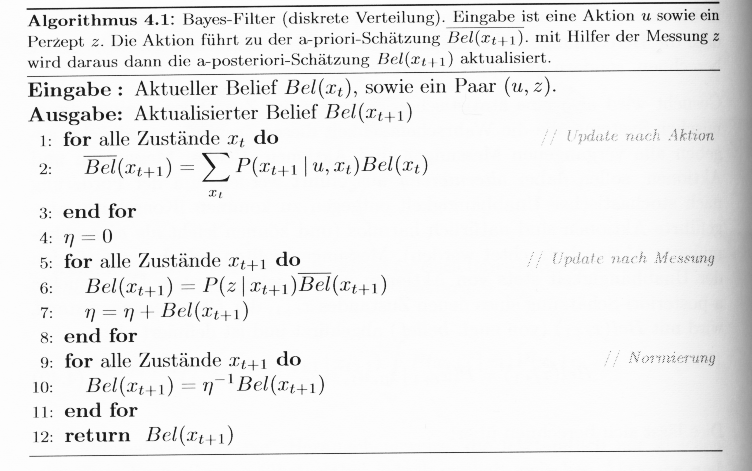
\includegraphics[scale=0.4]{Resources/PNG/hertzberg-132-bayes-algorithmus.png}
\end{center}

\subsection{Beispiel Aufgabenstellung}
Roboter schätzt den Zustand einer Tür mittels einer Kamera, er macht eien
Beobachtung z.

Annahmen:
\begin{itemize}
	\item Türe kann nur offen oder geschlossen sein
	\item Nur der Roboter kann den Zustand der Tür ändern
\end{itemize}

Der Roboter kennt den Zustand der Tür nicht $\Rightarrow$ Gleichverteilung
\begin{align*}
	&bel(X_0 = open) &= 0.5 \\
	&bel(x_0 = closed) &= 0.5
\end{align*}

Verrauschen der Sensoren $\Rightarrow$ bedingt Wahrscheinlichkeit
\begin{align*}
	&p(Z_t = sense\_open | X_t\, is\_open) = 0.6 \\
	&p(Z_t = sense\_closed | X_t\, is\_open) = 0.4 \\
	&p(Z_t = sense\_open | X_t\, is\_closed) = 0.2 \\
	&p(Z_t = sense\_closed | X_t\, is\_closed) = 0.8
\end{align*}

Der Roboter kann die Tür öffnen
\begin{align*}
	&p(X_t = is\_open | U_t = push, X_{t-1} = is\_open) = 1 \\
	&p(X_t = is\_closed | U_t = push, X_{t-1} = is\_open) = 0 \\
	&p(X_t = is\_open | U_t = push, X_{t-1} = is\_closed) = 0.8 \\
	&p(X_t = is\_closed | U_t = push, X_{t-1} = is\_closed) = 0.2
\end{align*}

Der Roboter tut nichts
\begin{align*}
	&p(X_t = is\_open | U_t = nothing, X_{t-1} = is\_open) = 1 \\
	&p(X_t = is\_closed | U_t = nothing, X_{t-1} = is\_open) = 0 \\
	&p(X_t = is\_open | U_t = nothing, X_{t-1} = is\_closed) = 0 \\
	&p(X_t = is\_closed | U_t = nothing, X_{t-1} = is\_closed) = 1
\end{align*}

\subsection{Beispiel Rechnung}
Für $t=1$ mit $u_1$ = nothing und $z_1$ = sense_open:
\begin{align*}
	\overline{bel}&(x_1 = open) = \\
		&p(x_1 = open | u = nothing, x_0 = open)bel(x_0 = open) + \\
		&p(x_1 = open | u = nothing, x_0 = closed)bel(x_0 = closed) \\
		&= 1 * 0.5 + 0 * 0.5 = 0.5 \\
	\overline{bel}&(x_1 = closed) = \\
		&p(x_1 = closed | u = nothing, x_0 = open)bel(x_0 = open) + \\
		&p(x_1 = closed | u = nothing, x_0 = closed)bel(x_0 = closed) \\
		&= 0 * 0.5 + 1 * 0.5 = 0.5 \\
	\eta = 0: bel&(x_1 = open) =  \\
		&p(z = sense_open | x_1 = open)\overline{bel}(x_1 = open) \\
		&= 0.6 * 0.5 = 0.3 \\
	\eta = 0.3: bel&(x_1 = closed) = \\
		&p(z = sense_open | x_1 = closed)\overline{bel}(x_1 = closed)\\
		&= 0.2 * 0.5 = 0.1 \\
	\eta = 0.4: bel&(x_1 = open) = bel(x_1 = open) * \eta^-1
		= 0.3 * 0.4^-1 = 0.75 \\
	bel&(x_1 = closed) = bel(x_1 = closed) * \eta^-1
		= 0.1 * 0.4^-1 = 0.25
\end{align*}

{
\begin{wrapfigure}{r}{0.4\textwidth}
	\includegraphics[width=0.4\textwidth]{Resources/PNG/MarkovAlgorithmus.PNG}
\end{wrapfigure}
\section{Markov Lokalisierung}
Bei der Markov Lokalisierung geht von der Annahme aus, dass der nachfolgene
Zustand nur vom akuellen Zustand abhängt. Dafür bietet sich der Bayes-Filter an.
Dabei wird der Bayes-Filter auf das Lokalisierungsproblem angewendet. Dafür ist
als weitere Input die Karte notwendig. Für die Markov Lokalisierung ist eine
\textbf{möglichst genaues Umgebungsmodell} notwendet.

Der Algorithmus ist wie beim Bayes-Filter es wird nur die Karte m als
zusätzliches Parameter für die Wahrscheinlichkeit hinzugefügt.
\begin{align*}
	\overline{bel}(x_t) &= \int p(x_t | u_t, x_{t-1}, m)bel(x_{t-1})dx \\
	bel(x_t) &= \eta p(z_t | x_t, m)\overline{bel}(x_t)
\end{align*}

}

{
\begin{wrapfigure}{r}{0.4\textwidth}
	\includegraphics[width=0.4\textwidth]{Resources/PNG/MonteCarlo.PNG}
\end{wrapfigure}
\section{Monte Carlo Lokalisierung}
Die Monte Carlo Lokalisierung ist ein Stichprobenbasiertes
Approximationsverfahren für die Markov Lokalisierung. Der Bayes Filter wird
auch hier benutzt, unterschiedet sich jedoch von gridbasierten
Lokalisationsverfahren anhand der Betrachtung und Verarbeitung.

\paragraph{Praxis:} Viele der Gitterzellen besitzen Wahrscheinlichkeit von 0.
Diese Gitterzellen miteinzubeziehen ist ineffizient. Diese können vernachlässigt
werden.

}

\paragraph{Funktionsweise}
\begin{itemize}
	\item Positionsschätzung bei $(x_k)$ wird durch eine Menge von
		\textbf{Partikeln} dargestellt
	\item Es besteht keine Information über die Anfangsposition; Partikel sind
		\textbf{zufällig verteilt}
	\item Durch \textbf{Sensormessung $z$} werden die \textbf{Gewichte}
		(Strichhöhe) verändert
	\item \textbf{Resampling}: Aus der Partikelmenge werden mit gewichteten
	 	Zufall Partikel entzogen  $\Rightarrow$ Integrierung des Steuerbefehls
		$(u_k)$
	\item Es erfolgt eine erneute Gewichtung mit einem neuen Sensorwert
	\item Anschließend ein erneuetes Resamplung und Integrierung des Steuerbefehls
\end{itemize}

\paragraph{Vorteil}
\begin{itemize}
	\item zur Laufzeit kann die Größe der Stichprobenmenge variabel sein
	\item je unsicherer die Roboterposition ist, desto größer ist die
		Stichprobenmenge
\end{itemize}

\subsection{Partikelmengen}
\begin{itemize}
	\item Jeder Partikel stellt eine \textbf{Hypothese} für den \textbf{Zustand
		$x$} dar
	\item Generierung einer Partikelmenge X aus einer Wahrscheinlichkeitsichte p:
\end{itemize}
\begin{figure}[H]
	\begin{center}
		\includegraphics[scale=0.5]{Resources/PNG/PartikelMengen.PNG}
		\caption{Partikelmengen}
		\label{fig:PNG/PartikelMengen.PNG}
	\end{center}
\end{figure}

\section{Kalman-Filter}
\subsection{Definition}
\begin{itemize}
	\item Zustandsschätzer für dynamische Systeme
	\item Spezielle Version eines Bayes-Filters
	\item Dient zur Fusion von zwei unterschiedlichen, stochastisch unabhängigen
		Informationsquellen
\end{itemize}

\textbf{Anwendung} fusion der Odometriedaten mit externen Messungen

\subsection{Vorgehen}
\begin{itemize}
	\item $Bel(x_t)$ wird durch seinen Erwartungswert $\mu$ sowie die Kovarianz
		$\sum_t$ approximiert.
	\item Zu jedem Zeitpunkt wird eine \textbf{Zustandsschätzung} geliefert, die
		aus einer Schätzung des aktuellen Zustandes und aus einer Vorhersage des
		Nachfolgezustandes nach Ausführung einer Aktion besteht.
	\item In die \textbf{Zustandsschätzungen} werden unabhängige Sensormessungen
		integriert
	\item In der \textbf{Vorhersagephase} benutzt der Kalman Filter die
		Zustandsschätzung vom vorhergehenden Zeitschritt um Zustandsschätzung für
		den aktuellen Zeitschritt zu erzeugen
	\item In der \textbf{Update} oder \textbf{Korrekturphase} werden die
		Messinformationen des aktuellen Zeitschritts verwendet, um die Vorhersage
		zu verbessern.
	\item Das Fehler Modell der Schätzung soll optimal aktualisiert werden auf
		Basis vorhandener Informationen
\end{itemize}

\subsection{Einschränkungen}
\begin{itemize}
	\item Fehlermodelle sind Gaußverteilungen
	\item Die Zustandsverteilung ist eine Gaußverteilung
\end{itemize}
\begin{figure}[H]
	\begin{center}
		\includegraphics[scale=0.4]{Resources/PNG/KalmanFilter.PNG}
		\caption{Kalman Filter}
		\label{fig:PNG/KalmanFilter.PNG}
	\end{center}
\end{figure}
\begin{itemize}
	\item \textbf{Links}: Unsicherheit im aktuellen Zustand x
	\item \textbf{Mitte}: eine unabhängige Messung z liefert konkurrierende
		Informationen (\textit{Mittelwewrt und Varianz})
	\item \textbf{Rechts:} Fusion beider Daten liefert eine Mittelung, gewichtet
		mit der Sicherheit der Informationen, sowie reduzierte Varianz, d.h. eine
		größere Sicherheit in dem gefilterten Zustand
\end{itemize}

\section{Simultaneous Localization and Mapping (SLAM)}
\subsection{Landmarkenbasiertes SLAM Problem}
\begin{itemize}
	\item \textbf{Ausgangspunkt} Roboter exploriert eine unbekannte, statistische
		Umgebung
	\subitem Roboter kennt seine Pose (Position und Orientierung) nicht genau
	\subitem Es existiert keine Karte der Umgebung
	\item \textbf{Bekannt} sind Sensor- und Steuerdaten: $d = u_1, z_1, u_2, z_2
		... u_k, z_k$
	\item \textbf{Gesucht} Karte $m$ mit $M$ Landmarken: $m = l_1, x, l_1, y,
		..., l_M,x,l_M,y$
	\subitem Weg des Roboters $x_1, x_2, ... x_k$
\end{itemize}

\paragraph{Probabilistische Algorithmen}
Ungenauigkeiten in den Messdaten werden durch Wahrscheinlichkeitsverteilungen
modelliert
\begin{itemize}
	\item bekannt sind die \textbf{Roboter Bewegungsbefehle} (die Kontrolldaten,
		die Steuerkommandos $u_t$)
	\item bekannt sind die \textbf{Beobachtungen} $z_t$ der nahe gelegnen
		\textbf{Landmarken} bestehend aus Entfernung und Winkel
	\item die Sensorik kann sowohl die Beobachtungsrichtung als auch die
		beobachtete Entfernung einer Landmarke zur Verfügung stellen
	\item gesucht ist eine Schätzung der Karte der Merkmale, der
		Landmarkenpositionen, sowie der Pfad des Roboters, d.h. seine aktuelle und
		frühere Posen
\end{itemize}

\subsection{Problemstellung}
\begin{itemize}
	\item Roboterpfad und Positionen der Landmarken in der Karte sind unbekannt
	\item Die Zuodnung von Messdaten zu Landmarken sind i.d. Regel unbekannt
	\item Roboter muss entscheiden, ob Messdaten einer bereits beobachteten
		Landmarke zugeordnet werden können oder einer noch nicht gesehenen Landmarke
	\item Problematik der Zuordnung wird durch Unsicherheit in der
		Roboterposition verstärkt
\end{itemize}
\begin{figure}[H]
	\begin{center}
		\includegraphics[scale=0.5]{Resources/PNG/ProbabilisitischeLandmarken.PNG}
		\caption{}
		\label{fig:PNG/ProbabilistischeLandmarken.PNG}
	\end{center}
\end{figure}

\subsection{Funktionsweise}
\begin{figure}[H]
	\begin{center}
		\includegraphics[scale=0.5]{Resources/PNG/FunktionsweiseSLAM.PNG}
		\caption{SLAM Darstellung}
		\label{fig:PNG/FunktionsweiseSLAM.PNG}
	\end{center}
\end{figure}
\begin{itemize}
	\item \textbf{(a)} Roboter misst Distanzen zu den Landmarken
	\item \textbf{(b)} Roboter schätzt seine neue Position anhand von Odometriedaten; Odometrie-basierte Roboterpose kann zur Schätzung der neuen Distanzen zu den in \textbf{(a)} verwendeten Landmarken herangezogen werden
	\item Nach Vergleich zwischen Roboter und Landmarken kann der Roboter seine Position \textbf{(c)} korrigieren
\end{itemize}

\subsection{Hinzunahme neuer Landmarken}
\begin{figure}[H]
	\begin{center}
		\includegraphics[scale=0.3]{Resources/PNG/LandmarkenErweitern.PNG}
		\caption{}
		\label{fig:PNG/LandmarkenErweitern.PNG}
	\end{center}
\end{figure}
\begin{itemize}
	\item (a) entspricht der Situation aus der vorhergehenden Folie.
	\item In (b) lokalisiert sich das Fahrzeug nach einer Bewegung erneut anhand
		zweier \enquote{alter} Landmarken und der letzten lokalen Karte
	\item Führt aufgrund der Fehler zu einer ungenauen, globalen Roboterposition
	\item Die Position der neuen Landmarken wird relativ zu der vermeintlich
		bekannten, korrekten Position der alten Landmarken bestimmt
	\item Positionsannahme ist inkorrekt
	\item Verschiebung der Position der \enquote{alten} Landmarken wird geschätzt
		und korrigiert sowie auf die Position der neuen Landmarken angewandt
\end{itemize}

\subsection{Aufbau eines SLAM-Graphen}
\begin{itemize}
	\item Sämtliche Messvorgänge sind fehlerbehaftet, auch die
		Positionsbestimmung der Landmarken
	\item Die Unsicherheit wird in der folgenden Abbildung als Fehlerellipse
		dargestellt.
	\item Roboter schätzt die Landmarken \textbf{A} und \textbf{B}
	\item nach Bewegung des Roboters nimmt die Genauigkeit der Lokalisierung ab
	\item Die Unsicherheit der Positionsschätzung der Landmarken \textbf{C} und
		\textbf{D} steigt
	\item Der Roboter erkennt eine bereits zuvor gesehene Landmarke
	\item Eine Verknüpfung mit der früheren Information über die Landmarke
		reduziert die Unsicherheit bei der Positionsbestimmung und damit auch die
		Unsicherheit über die zugehörigen früheren Roboterpositionen
\end{itemize}
\begin{minipage}[]{0.5\textwidth}
\begin{figure}[H]
	\begin{center}
		\includegraphics[scale=0.32]{Resources/PNG/LandmarkenBeispiel.PNG}
		\caption{}
		\label{fig:PNG/LandmarkenBeispiel.PNG}
	\end{center}
\end{figure}
\end{minipage}
\begin{minipage}[]{0.5\textwidth}
\begin{figure}[H]
	\begin{center}
		\includegraphics[scale=0.3]{Resources/PNG/LandmarkenBeispiel2.PNG}
		\caption{}
		\label{fig:PNG/LandmarkenBeispie2l.PNG}
	\end{center}
\end{figure}
\end{minipage}

\subsection{Varianten von SLAM}
\paragraph{Vollständiges SLAM}
\begin{itemize}
	\item Roboter schätzt eine Umgebungskarte $m$
	\item Roboter schätzt seine aktuelle Pose $x_t$ und \textbf{alle}
		zurückliegenden Posen $x_t-1$ bis $x_1$
	\item Grundlage sind die bisher wahrgenommenen Sensordaten $z_1:t$
	\item Sowie alle ausgeführten Aktionen $u_1:t-1$
	\item Es muss die Verteilung $P(m, x1:t | z_1:t, u1:t-1)$
\end{itemize}

\paragraph{Inkrementelles Slam}
\begin{itemize}
	\item Roboter schätzt nur die Karte $m$ sowie die aktuelle Position $x_t$
	\item Es muss die Verteilung $P(m, x_t | z1:t, u1:t-1)$ geschätzt werden
\end{itemize}

\subsection{Bayesian Netzwerk für landmarkenbasiertes SLAM}
\begin{itemize}
	\item Die einzelnen Landmarken sind unabhängig
	\item Gegeben sind die Roboterposen
\end{itemize}
\begin{figure}[H]
	\begin{center}
		\includegraphics[scale=0.5]{Resources/PNG/BayesNetzwerk}
		\caption{Bayes Netzwerk}
		\label{fig:PNG/BayesNetzwerk}
	\end{center}
\end{figure}
Modell von Variablen und deren Abhängigkeiten als dynamisches Bayes-Netzwerk.
\begin{itemize}
	\item Kern des Modells bilden die
		\subitem Zeitreihe der Roboterzustände $s_1, s_2, ... s_t$
		\subitem die Positionen der Landmarken $\theta_k$
		\subitem die Kontrollvariablen $u_t$
		\subitem und die gemessenen, beobachteten Landmarken Positionen $z_t$
	\item Der Roboter bewegt sich von $s_1$ nach $s_t$ mit einer Folge
		Kontrolleingaben $u_2, ... u_t$
	\item Der Roboterzustand $s_t$ zum Zeitpunkt $t$ ist lediglich vom
		Roboterzustand $s_t-1$ zum vorhergehenden Zeitpunkt und dem ausgeführten
		Steuerkommando $u_t$ des Roboters abhängig
	\item Zum Zeitpunkt $t = 1$ beobachtet der Roboter die Landmarkenpositionen
		$\theta_1$ mittels $z_1$ zum Zeitpunkt $t = 2$ beobachtet er $\theta_2$ via
		$z_2$ und zum Zeitpunkt $t = 3$ wieder $\theta_1$
	\item Die Beobachtung $z_t$ ist abhängig von der globalen Position der
		Landmarke $\theta_k$ und dem aktuellen Roboterzustand $s_t$
	\item \textbf{FastSLAM} zerlegt das Problem
		\subitem in die \textbf{Lokalisation} (Wissen über den vom Roboter
			zurückgelegten weg  $s_1, ... s_t$)
		\subitem und einer Sammlung von einzelnen \textbf{Landmarken-schätzungen}
			$z_k$, die von der geschätzter Roboterpose abhängen
	\item Zeitkomplexität von \textbf{FastSLAM} ist $O(f M)$
		\subitem $f$ konstanter Faktor
		\subitem $M$ Anzahl der Landmarken
\end{itemize}
